\documentclass[11pt]{beamer}
%\documentclass[11pt, handout]{beamer}

% Allgemeine Definitionen
\usepackage[english]{babel}	% Deutsche Sprachanpassung, z.B. Silbentrennung bei Worten mit Sonderzeichen
\usepackage[utf8]{inputenc}		% Direkte Eingabe von Umlauten

\usepackage{multimedia}		% Animations-Unterstützung (braucht hyperref | hyperref ist Teil von beamer )

% Verschiedene Operatoren
\newcommand{\union}{\ensuremath{\cup}}		% Die Vereinigung
\newcommand{\schnitt}{\ensuremath{\cap}}		% Der Schnitt
\newcommand{\und}{\ensuremath{\wedge}}		% Das und-Symbol
\newcommand{\oder}{\ensuremath{\vee}}		% Das oder-Symbol
\newcommand{\folgt}[1]{\ensuremath{\stackrel{#1}{\Rightarrow}}}	% Das Folgerungszeichen mit Symbol darüber 
\newcommand{\gleich}[1]{\ensuremath{\stackrel{#1}{=}}}	% Das Gleichheitszeichen mit Symbol darüber 
\newcommand{\isdef}{\ensuremath{\mathrel{\mathop:}=}}		% Das "ist-definiert"-Zeichen
\newcommand{\defis}{\ensuremath{=\mathrel{\mathop:}}}		% Das "ist-definiert"-Zeichen (andersrum)

% Weiterer nützlicher Kram
%\usepackage{enumitem}		% NICHT kompatibel mit beamer!
\usepackage{amsfonts, amsmath, amssymb}
\usepackage{amsthm}			% Eigene Umgebungen
\usepackage{thumbpdf}	% Seitenvorschau in PDF-Dokumenten

\usepackage{nicefrac}

\usepackage{pgf, tikz}
\usetikzlibrary{arrows, decorations.pathreplacing, calc}

% Erst die Farbe (optional), dann die Norm, dann der Inhalt
\newcommand{\norm}[3][black]{\ensuremath{\left\Vert #3\right\Vert_{\textcolor{#1}{#2}}}}

% Die folgenden Befehle dienen dazu, verschiedene Konventionen darzustellen. Man kann damit
% auf einfache Weise die in dem Dokument verwendeten Konventionen umschalten.

%\newcommand{\bisn}[1]{\ensuremath{\underline{#1}}}	% Bezeichnung für die Menge {1,..,n}
\newcommand{\bisn}[1]{\ensuremath{\{1,\dots , #1 \}}}	% Alternative (ohne Fallunterscheidung)

% Das Erzeugnis, das erste Argument zeigt an, welches Erzeugnis gemeint ist, das zweite gibt seinen Inhalt an.
%\newcommand{\spn}[2][]{\ensuremath{\mathrm{span} \{ #1 \}}}
\newcommand{\spn}[2][]{\ensuremath{\left\langle #2 \right\rangle _{ #1 }}}

\newcommand{\grad}[1]{\ensuremath{\mathrm{grad}( #1 )}}
%\newcommand{\grad}[1]{\ensuremath{\nabla #1}}

\newcommand{\tr}[1]{\ensuremath{#1^{tr}}} % Bezeichnung für die Transponierte einer Matrix

% Die Mengentheoretische Differenz
\newcommand{\ohne}{\ensuremath{-}}
%\newcommand{\ohne}{\ensuremath{\backslash}}

\DeclareMathOperator{\Hom}{Hom}
\DeclareMathOperator{\GL}{GL}
\DeclareMathOperator{\diag}{diag}
\DeclareMathOperator{\Rg}{Rang}
\DeclareMathOperator{\Bild}{Bild}
\DeclareMathOperator{\Kern}{Kern}
\DeclareMathOperator{\Spur}{Spur}
\DeclareMathOperator{\Aut}{Aut}
\DeclareMathOperator{\Sym}{Sym}
\DeclareMathOperator{\Pot}{Pot}
\DeclareMathOperator{\Grad}{Grad}
\DeclareMathOperator{\kgV}{kgV}

\newcommand{\menge}[1]{\ensuremath{\mathbb{#1}}}
\newcommand{\N}{\menge{N}}
\newcommand{\Z}{\menge{Z}}
\newcommand{\Q}{\menge{Q}}
\newcommand{\R}{\menge{R}}
\newcommand{\C}{\menge{C}}

% Mit den schönen Buchstaben arbeiten
\renewcommand{\phi}{\varphi}

\renewcommand{\subset}{\subseteq}

% Verschiedene mögliche Umgebungen
\newtheorem{lem}{Lemma}[section]		% Lemma
\newtheorem{bsp}[lem]{Beispiel}		% Beispiel
\newtheorem{folg}[lem]{Folgerung}	% Folgerung
\newtheorem{bem}[lem]{Bemerkung}
\newtheorem{satz}[lem]{Satz}			% Satz
\newtheorem{kor}[lem]{Korollar}		% Korollar
%\newtheorem{alg}[lem]{Algorithmus}	% Algorithmus
%\theoremstyle{definition}
\newtheorem{defi}[lem]{Definition}	% Definition
\theoremstyle{remark}
\newtheorem*{idea}{Beweisidee}	% Beweisidee (vor dem eigentlichen Beweis)




\beamertemplatenavigationsymbolsempty

\usetheme{Madrid}
%	AnnArbor | Antibes | Bergen |
%	Berkeley | Berlin | Boadilla |
%	boxes | CambridgeUS | Copenhagen |
%	Darmstadt | default | Dresden |
%	Frankfurt | Goettingen |Hannover |
%	Ilmenau | JuanLesPins | Luebeck |
%	Madrid | Malmoe | Marburg |
%	Montpellier | PaloAlto | Pittsburgh |
%	Rochester | Singapore | Szeged |
%	Warsaw
%\usecolortheme{seahorse}
%	albatross | beaver | beetle |
%	crane | default | dolphin |
%	dove | fly | lily | orchid |
%	rose |seagull | seahorse |
%	sidebartab | structure |
%	whale | wolverine
%\usefonttheme{professionalfonts}
%	default | professionalfonts | serif |
%	structurebold | structureitalicserif |
%	structuresmallcapsserif
%\useinnertheme{rounded}
%	circles | default | inmargin |
%	rectangles | rounded
%\useoutertheme{shadow}
%	default | infolines | miniframes |
%	shadow | sidebar | smoothbars |
%	smoothtree | split | tree

% Graphic support
\newcommand{\primaryBlue}{blue}
\newcommand{\primaryRed}{red}
\newcommand{\primaryGreen}{green!60!black}
\newcommand{\primaryYellow}{yellow}


\newcommand{\colorVertex}{\primaryBlue!50!white}
\newcommand{\colorEdge}{black}
\newcommand{\colorFace}{\primaryYellow}
\newcommand{\colorDarkFace}{\primaryYellow!80!black}
\newcommand{\colorEdgeBack}{magenta!20!white}

\newcommand{\colorVertexNode}{\colorVertex}

\newcommand{\colorEdgeA}{\primaryBlue}
\newcommand{\colorEdgeB}{\primaryRed}
\newcommand{\colorEdgeC}{\primaryGreen}


\newcommand{\colorFaceA}{cyan}
\newcommand{\colorFaceB}{magenta}
\newcommand{\colorFaceC}{orange}

\newcommand{\colorRed}{\primaryRed}


\newcommand{\graphColorA}{purple}
\newcommand{\graphColorB}{\primaryGreen}
\newcommand{\graphColorC}{orange}
\newcommand{\graphColorD}{black}
\newcommand{\graphColorE}{\primaryBlue}

\newcommand{\colorGraphA}{\graphColorA}
\newcommand{\colorGraphB}{\graphColorB}
\newcommand{\colorGraphC}{\graphColorE}

\newcommand{\colorGraphAlpha}{\graphColorB}
\newcommand{\colorGraphBeta}{\graphColorE}
\newcommand{\colorGraphGamma}{\graphColorC}
\newcommand{\colorGraphDelta}{\graphColorD}

% This document contains the TikZ-header for all our LaTeX-computations.
% It especially contains all global graphic parameters.

\usepackage{amsmath, amssymb, amsfonts} % Standard Math-stuff

\usepackage{tikz}
\usetikzlibrary{calc}
\usetikzlibrary{positioning}
\usetikzlibrary{shapes}
\usetikzlibrary{patterns}

% Define a text=none option for nodes that ignores the given text, from
% https://tex.stackexchange.com/questions/59354/no-text-none-in-tikz
\makeatletter
\newif\iftikz@node@phantom
\tikzset{
  phantom/.is if=tikz@node@phantom,
  text/.code=%
    \edef\tikz@temp{#1}%
    \ifx\tikz@temp\tikz@nonetext
      \tikz@node@phantomtrue
    \else
      \tikz@node@phantomfalse
      \let\tikz@textcolor\tikz@temp
    \fi
}
\usepackage{etoolbox}
\patchcmd\tikz@fig@continue{\tikz@node@transformations}{%
  \iftikz@node@phantom
    \setbox\pgfnodeparttextbox\hbox{}
  \fi\tikz@node@transformations}{}{}
\makeatother

% Now we define the global styles
% The global styles are defined nestedly. You have to give your tikzpicture
% the global options [vertexStyle, edgeStyle, faceStyle] to activate them.
% 
% You can disable labels by using the option nolabels, i.e. 
% vertexStyle=nolabels to deactivate vertex labels.
%
% If you want to have a specific style for your picture, you can also use
% this specific meta-style instead of the general style. For example if you
% want to use double edges in one single picture - no matter the style of
% the rest of the document - you can use edgeDouble instead of edgeStyle.
%
% To set the default style, modify the vertexStyle/.default entry.

% Vertex styles
\tikzset{ 
    vertexNodePlain/.style = {fill=gray, shape=circle, inner sep=0pt, minimum size=2pt, text=none},
    vertexPlain/labels/.style = {
        vertexNode/.style={vertexNodePlain},
        vertexLabel/.style={gray}
    },
    vertexPlain/nolabels/.style = {
        vertexNode/.style={vertexNodePlain},
        vertexLabel/.style={text=none}
    },
    vertexPlain/.style = vertexPlain/#1,
    vertexPlain/.default=labels
}
\tikzset{
    vertexNodeNormal/.style = {fill=blue, shape=circle, inner sep=0pt, minimum size=4pt, text=none},
    vertexNormal/labels/.style = {
        vertexNode/.style={vertexNodeNormal},
        vertexLabel/.style={blue}
    },
    vertexNormal/nolabels/.style = {
        vertexNode/.style={vertexNodeNormal},
        vertexLabel/.style={text=none}
    },
    vertexNormal/.style = vertexNormal/#1,
    vertexNormal/.default=labels
}
\tikzset{
    vertexNodeBall/.style = {shape=circle, ball color=orange, inner sep=2pt, outer sep=0pt, minimum size=3pt, font=\tiny},
    vertexBall/labels/.style = {
        vertexNode/.style={vertexNodeBall, text=black},
        vertexLabel/.style={text=none}
    },
    vertexBall/nolabels/.style = {
        vertexNode/.style={vertexNodeBall, text=none},
        vertexLabel/.style={text=none}
    },
    vertexBall/.style = vertexBall/#1,
    vertexBall/.default=labels
}
\tikzset{ 
    vertexStyle/.style={vertexNormal=#1},
    vertexStyle/.default = labels
}


% 1) position of the vertex
% 2) relative position of the node
% 3) name of the vertex
\newcommand{\vertexLabelR}[3]{
    \node[vertexNode] at (#1) {#3};
    \node[vertexLabel, #2] at (#1) {#3};
}
% 1) position of the vertex
% 2) absolute position of the node
% 3) name of the vertex
\newcommand{\vertexLabelA}[3]{
    \node[vertexNode] at (#1) {#3};
    \node[vertexLabel] at (#2) {#3};
}


% Edge styles
% If you have trouble with the double-lines overlapping, this might (?) help:
% https://tex.stackexchange.com/questions/288159/closing-the-ends-of-double-line-in-tikz
\newcommand{\edgeLabelColor}{blue!20!white}
\tikzset{
    edgeLineNone/.style = {draw=none},
    edgeLineNone/.default=black,
    edgeNone/labels/.style = {
        edge/.style = {edgeLineNone=##1},
        edgeLabel/.style = {fill=\edgeLabelColor}
    },
    edgeNone/nolabels/.style = {
        edge/.style = {edgeLineNone=##1},
        edgeLabel/.style = {text=none}
    },
    edgeNone/.style = edgeNone/#1,
    edgeNone/.default = labels
}
\tikzset{
    edgeLinePlain/.style={line join=round, draw=#1},
    edgeLinePlain/.default=black,
    edgePlain/labels/.style = {
        edge/.style={edgeLinePlain=##1},
        edgeLabel/.style={fill=\edgeLabelColor}
    },
    edgePlain/nolabels/.style = {
        edge/.style={edgeLinePlain=##1},
        edgeLabel/.style={text=none}
    },
    edgePlain/.style = edgePlain/#1,
    edgePlain/.default = labels
}
\tikzset{
    edgeLineDouble/.style = {thin, double=#1, double distance=.6pt, line join=round},
    edgeLineDouble/.default=gray!90!white,
    edgeDouble/labels/.style = {
        edge/.style = {edgeLineDouble=##1},
        edgeLabel/.style = {fill=\edgeLabelColor}
    },
    edgeDouble/nolabels/.style = {
        edge/.style = {edgeLineDouble=##1},
        edgeLabel/.style = {text=none}
    },
    edgeDouble/.style = edgeDouble/#1,
    edgeDouble/.default = labels
}
\tikzset{
    edgeStyle/.style = {edgePlain=#1},
    edgeStyle/.default = labels
}

% Face styles
% Here we have an exception - the style face is always defined.
% 
\newcommand{\faceColorY}{yellow!60!white}   % yellow
\newcommand{\faceColorB}{blue!60!white}     % blue
\newcommand{\faceColorC}{cyan!60}           % cyan
\newcommand{\faceColorR}{red!60!white}      % red
\newcommand{\faceColorG}{green!60!white}    % green
\newcommand{\faceColorO}{orange!50!yellow!70!white} % orange

% define default face colour (and default swap colour)
\newcommand{\faceColor}{\faceColorY}
\newcommand{\faceColorSwap}{\faceColorC}

% define secondary default colours (to use in a single section)
\newcommand{\faceColorFirst}{green!40!white}
\newcommand{\faceColorSecond}{gray!15!white}
\newcommand{\faceColorThird}{red!17!white}
\newcommand{\faceColorFourth}{olive!20!white}

\tikzset{
    face/.style = {fill=#1},
    face/.default = \faceColor,
    faceY/.style = {face=\faceColorY},
    faceB/.style = {face=\faceColorB},
    faceC/.style = {face=\faceColorC},
    faceR/.style = {face=\faceColorR},
    faceG/.style = {face=\faceColorG},
    faceO/.style = {face=\faceColorO}
}
\tikzset{
    faceStyle/labels/.style = {
        faceLabel/.style = {}
    },
    faceStyle/nolabels/.style = {
        faceLabel/.style = {text=none}
    },
    faceStyle/.style = faceStyle/#1,
    faceStyle/.default = labels
}
\tikzset{ face/.style={fill=#1} }
\tikzset{ faceSwap/.code=
    \ifdefined\swapColors
        \tikzset{face=\faceColorSwap}
    \else
        \tikzset{face=\faceColor}
    \fi
}

% Sometimes we want to implement different behaviour for the generated 
% HTML-pictures (for example, shading is not supported in HTML).
% For that we define a macro to check whether we run the code with
% htlatex. The code comes from 
% https://tex.stackexchange.com/questions/93852/what-is-the-correct-way-to-check-for-latex-pdflatex-and-html-in-the-same-latex
\makeatletter
\edef\texforht{TT\noexpand\fi
  \@ifpackageloaded{tex4ht}
    {\noexpand\iftrue}
    {\noexpand\iffalse}}
\makeatother


\usepackage{hyperref}



\author[M. Baumeister]{Markus Baumeister\\ \vspace{1mm} \small{(j/w Alice Niemeyer, Wilhelm Plesken, Ansgar Strzelczyk)}}
\title{Simplicial surfaces}
\institute[RWTH Aachen]{Lehrstuhl B für Mathematik\\RWTH Aachen University}
\date{27.09.2017}

\begin{document}

% Titelseite
\begin{frame}
\titlepage
\end{frame}



\begin{frame}{Simplicial surfaces}
    \pause
        \begin{center}
            \begin{tikzpicture}[scale=2]
    \begin{scope}[scale=0.5,yshift=0.8cm]
                    % Coordinates of octahedron
                \def\len{2} % The length of the base
                \def\h{0.9}   % \h*\len is the hight of the apex above the 
                            % center of the square
                \coordinate (Mid) at (0,0);
                \coordinate (Right) at (0.5*\len,0.3*\len);
                \coordinate (Left) at (-0.75*\len,0.25*\len);
                \coordinate (Back) at ($(Right)+(Left)$);
                \coordinate (Center) at ($(Left)!0.5!(Right)$);
                \coordinate (Up) at ($(Center)+(0,\h*\len)$);
                \coordinate (Down) at ($(Center)+(0,-\h*\len)$);

                \filldraw[face] (Up) -- (Mid) -- (Left) -- cycle;
                \filldraw[face] (Up) -- (Mid) -- (Right) -- cycle;
                \filldraw[face] (Down) -- (Mid) -- (Left) -- cycle;
                \filldraw[face] (Down) -- (Mid) -- (Right) -- cycle;
                \draw[dashed] (Up) -- (Back) -- (Down);
                \draw[dashed] (Left) -- (Back) -- (Right);

 

    \end{scope}
    
    \begin{scope}[xshift=1cm]
        			    \coordinate (A) at (0,0);
			    \coordinate (B) at (1.7,0.5);
			    \coordinate (C) at (1.3,1.4);
			    \coordinate (D) at (0.5,1.5);
			    \coordinate (E) at (1,0.7);
			
			    % Take care to draw the faces in the back first
                            \draw[face,edge]
                                (A) -- (B) -- (C) -- cycle
                                (A) -- (C) -- (D) -- cycle;
                            \draw[face,edge]
                                (A) -- (B) -- (E) -- cycle
                                (A) -- (E) -- (D) -- cycle;
                            \draw[edge, dashed] (A) -- (C);

    \end{scope}

    \begin{scope}[xshift=3.5cm]
        			    \coordinate (A) at (0,0);
			    \coordinate (B) at (1.3,0.4);
			    \coordinate (C) at (0.4,1.3);
			
			    \filldraw[face] (A) -- (B) to[bend right=45] (C) -- cycle;
			    \filldraw[face] (A) -- (B) to[bend left=45] (C) -- cycle;


    \end{scope}
\end{tikzpicture}


        \end{center}
    
    \pause
    $\leadsto$ structures build from triangles
    \pause
    (or arbitrary polygons)
\end{frame}



\begin{frame}{Classification}
    \pause
    Goal: Classify all closed simplicial surfaces.

    \pause
    Plesken/Strzelczyk classified the building blocks up to 20 triangles.

    \begin{itemize}
        \pause
        \item e.\,g. exactly 87 non--isomorphic surfaces with 20 triangles
        \pause
        \item e.\,g. only one surface with 10 triangles:
    \end{itemize}

    \pause
    \begin{center}
        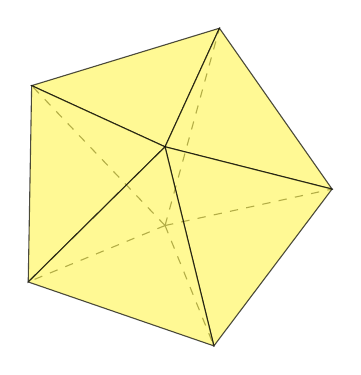
\begin{tikzpicture}[z={(0cm,1cm)},x={(-1cm,-1cm)},y={(1cm,-1cm)}, faceOp/.style={opacity=0.7}]
            \def\len{1.5}
            \def\h{0.5}

            \coordinate (Top) at (0,0,\h);
            \coordinate (Bottom) at (0,0,-\h);
            \foreach \i in {0,...,4}{
                \coordinate (P\i) at (-10+72*\i:\len);
            }

            \foreach \i in {0,...,4}{
                \draw[dashed] (Bottom) -- (P\i);
            }

            \filldraw[face,faceOp] (Top) -- (P3) -- (P4) -- cycle;
            \filldraw[face,faceOp] (Top) -- (P2) -- (P3) -- cycle;
            \filldraw[face,faceOp] (Top) -- (P4) -- (P0) -- cycle;
            \filldraw[face,faceOp] (Top) -- (P1) -- (P2) -- cycle;
            \filldraw[face,faceOp] (Top) -- (P0) -- (P1) -- cycle;

        \end{tikzpicture}
    \end{center}
\end{frame}



\newcommand{\colA}{\colorEdgeA}
\newcommand{\colB}{\colorEdgeB}
\newcommand{\colC}{\colorEdgeC}
\newcommand{\width}{very thick}

\begin{frame}{One type of triangle}
    \pause
    We are interested in surfaces that are built from one type of triangle.

    \pause
    \begin{center}
                %       F
                %    C     E 
                % A     B    D
                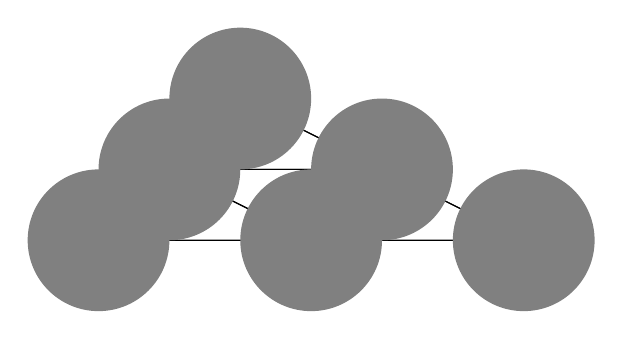
\begin{tikzpicture}[scale=0.9]
                    \coordinate (A) at (0,0);
                    \coordinate (B) at (3,0);
                    \coordinate (C) at (1,1);
                    \coordinate (D) at ($2*(B)$);
                    \coordinate (E) at ($(B)+(C)$);
                    \coordinate (F) at ($2*(C)$);

                        \draw (A) -- (B) -- (D) -- (E) -- (B) -- (C) -- (E) -- (F) -- (C) -- (A);

                        \draw[\colA, \width] (A) -- (B) -- (D);
                        \draw[\colA, \width] (C) -- (E);
                        \draw[\colB, \width] (B) -- (C);
                        \draw[\colB, \width] (D) -- (E) -- (F);
                        \draw[\colC, \width] (A) -- (C) -- (F);
                        \draw[\colC, \width] (B) -- (E);

                        \foreach \p in {A,B,C,D,E,F}
                            \fill[gray] (\p) circle (\vSize);
                \end{tikzpicture}
            \end{center}

    \pause
    $\leadsto$ edge--colouring encodes lengths

    \pause
    $\leadsto$ analyse edge--coloured surfaces
\end{frame}


\begin{frame}{Colouring as permutation}
    \onslide<2->{
        Consider a tetrahedron \onslide<3->{with an edge colouring}
    }
    \begin{center}
        \begin{tikzpicture}[scale=0.8]
                \coordinate (A) at (0,0);
                \coordinate (B) at (2,0);
                \coordinate (C) at (1,1.4);
                \coordinate (D) at ($2*(B)$);
                \coordinate (E) at ($(B)+(C)$);
                \coordinate (F) at ($2*(C)$);
            \onslide<2->{
                \draw (A) -- (B) -- (D) -- (E) -- (F) -- (C) -- (E) -- (B) -- (C) -- (A);
                \node at (barycentric cs:A=1,B=1,C=1) {1};
                \node at (barycentric cs:B=1,C=1,E=1) {2};
                \node at (barycentric cs:B=1,D=1,E=1) {3};
                \node at (barycentric cs:C=1,E=1,F=1) {4};
                \draw[dotted,thick] ($(A)!0.5!(C)$) to[bend left] ($(C)!0.5!(F)$);
                \draw[dotted,thick] ($(A)!0.5!(B)$) to[bend right] ($(B)!0.5!(D)$);
                \draw[dotted,thick] ($(D)!0.5!(E)$) to[bend right] ($(E)!0.5!(F)$);
            }
            \onslide<3->{
                \draw[\colA, \width] (A) -- (B) -- (D);
                \draw[\colA, \width] (C) -- (E);
                \draw[\colB, \width] (B) -- (C);
                \draw[\colB, \width] (D) -- (E) -- (F);
                \draw[\colC, \width] (A) -- (C) -- (F);
                \draw[\colC, \width] (B) -- (E);

                \foreach \p in {A,B,C,D,E,F}
                    \fill[gray] (\p) circle (\vSize);
            }

            % Draw switching arrows
            \onslide<7-9>{
                \draw[<->,\colB, thick] (barycentric cs:A=1,B=2,C=2) to[bend left] (barycentric cs:B=2,C=2,E=1);
            }
            \onslide<8-9>{
                \draw[<->,\colB,thick] (barycentric cs:B=1,D=2,E=2) to[bend right=60] (barycentric cs:E=2,F=2,C=1);
            }
            \onslide<10>{
                \draw[<->,\colA,thick] (barycentric cs:A=2,B=2,C=1) to[bend right=60] (barycentric cs:B=2,D=2,E=1);
                \draw[<->,\colA,thick] (barycentric cs:C=2,E=2,B=1) to[bend left] (barycentric cs:C=2,E=2,F=1);
            }
            \onslide<11>{
                \draw[<->,\colC,thick] (barycentric cs:A=2,B=1,C=2) to[bend left=60] (barycentric cs:C=2,E=1,F=2);
                \draw[<->,\colC,thick] (barycentric cs:B=2,C=1,E=2) to[bend left] (barycentric cs:B=2,D=1,E=2);
            }
        \end{tikzpicture}
    \end{center}
    \onslide<4->{
        \textit{simplicial surface} $\Rightarrow$ \onslide<5->{two faces at each edge}
    
        \begin{itemize}
            \item<6->[$\leadsto$] every edge defines a transposition of incident faces
            \item<9->[$\leadsto$] every colour class defines a permutation of the faces
            \item<7-> \textcolor{\colB}{(1,2)}\onslide<8->{\textcolor{\colB}{(3,4)}}
                    \onslide<10->{, \textcolor{\colA}{(1,3)(2,4)}}
                    \onslide<11->{, \textcolor{\colC}{(1,4)(2,3)}}
            \item<12->[$\leadsto$] group theoretic considerations
        \end{itemize}
    }
\end{frame}
         

\begin{frame}[fragile]{Construction example}
    \onslide<2->{ $\textcolor{\colA}{\sigma_a} = \textcolor{\colA}{(1,2)(3,4)(5,6)(7,8)}$\\ }
    \onslide<2->{ $\textcolor{\colB}{\sigma_b} = \textcolor{\colB}{(1,4)(2,3)(5,8)(6,7)}$\\ }
    \onslide<2->{ $\textcolor{\colC}{\sigma_c} = \textcolor{\colC}{(1,5)(2,6)(3,7)(4,8)}$\\ }

    \onslide<3->{
    \begin{center}
    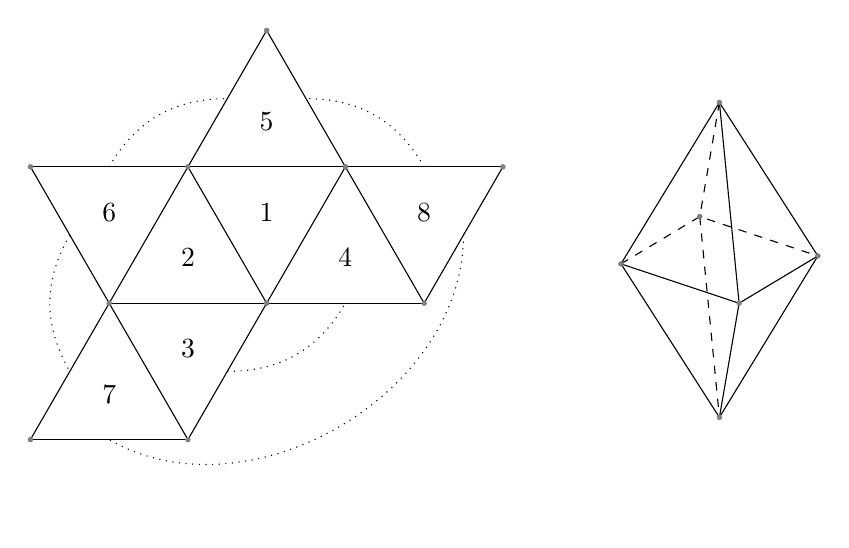
\begin{tikzpicture}
        % Coordinates
        \coordinate (Z) at (0,0);
        \foreach \i in {0,1,2,3,4}
            \coordinate (P\i) at (60*\i:2);
        \foreach \i/\j in {0/1, 1/2, 2/3, 3/4}
            \coordinate (Q\i\j) at ($(P\i)+(P\j)$);

        \newcommand{\vertex}[1]{
            \fill[black] (#1) circle (3pt);
        }


        % First vertex

        % 1
            \node at (barycentric cs:Z=1,P1=1,P2=1) {1};
            \draw[\colA,\width] (Z) -- (P2);
            \draw[\colB,\width] (Z) -- (P1);
            \draw[\colC,\width] (P1) -- (P2);

        % 2
            \node at (barycentric cs:Z=1,P2=1,P3=1) {2};
            \draw[\colB,\width] (Z) -- (P3);
            \draw[\colC,\width] (P2) -- (P3);

        % 3
            \node at (barycentric cs:Z=1,P3=1,P4=1) {3};
            \draw[\colC,\width] (P3) -- (P4);
            \draw[\colA,\width] (Z) -- (P4);

        % 4
            \node at (barycentric cs:Z=1,P0=1,P1=1) {4};
            \draw[\colA,\width] (Z) -- (P0);
            \draw[\colC,\width] (P0) -- (P1);

            \draw[\colA,\width,dotted] ($(Z)!0.5!(P4)$) to[bend right] ($(Z)!0.5!(P0)$);



        % Second vertex

        % 5
            \node at (barycentric cs:P1=1,P2=1,Q12=1) {5};
            \draw[\colB,\width] (P1) -- (Q12);
            \draw[\colA,\width] (P2) -- (Q12);

        % 6
            \node at (barycentric cs:P2=1,P3=1,Q23=1) {6};
            \draw[\colA,\width] (P2) -- (Q23);
            \draw[\colA,\width,dotted] ($(P2)!0.5!(Q23)$) to[bend left] ($(P2)!0.5!(Q12)$);
            \draw[\colB,\width] (P3) -- (Q23);


        % Third vertex

        % 7
            \node at (barycentric cs:P3=1,P4=1,Q34=1) {7};
            \draw[\colB,\width] (P3) -- (Q34);
            \draw[\colB,\width,dotted] ($(P3)!0.5!(Q23)$) to[bend right] ($(P3)!0.5!(Q34)$);
            \draw[\colA,\width] (P4) -- (Q34);


        % Fourth vertex

        % 8
            \node at (barycentric cs:P0=1,P1=1,Q01=1) {8};
            \draw[\colB,\width] (P1) -- (Q01);
            \draw[\colB,\width,dotted] ($(P1)!0.5!(Q01)$) to[bend right] ($(P1)!0.5!(Q12)$);
            \draw[\colA,\width] (P0) -- (Q01);


            \draw[\colA,\width,dotted] ($(P0)!0.5!(Q01)$) to[bend left=60] ($(P4)!0.5!(Q34)$);

        \foreach \p in {Z,P0,P1,P2,P3,P4,Q01,Q12,Q23,Q34}
            \fill[gray] (\p) circle (1pt);


        \begin{scope}[xshift=6cm]
            % Coordinates of octahedron
                \def\len{2} % The length of the base
                \def\h{1}   % \h*\len is the hight of the apex above the 
                            % center of the square
                \coordinate (Mid) at (0,0);
                \coordinate (Right) at (0.5*\len,0.3*\len);
                \coordinate (Left) at (-0.75*\len,0.25*\len);
                \coordinate (Back) at ($(Right)+(Left)$);
                \coordinate (Center) at ($(Left)!0.5!(Right)$);
                \coordinate (Up) at ($(Center)+(0,\h*\len)$);
                \coordinate (Down) at ($(Center)+(0,-\h*\len)$);

                \onslide<4>{
                    \draw[\colA,\width] (Up) -- (Mid) -- (Down);
                    \draw[\colA,\width,dashed] (Up) -- (Back) -- (Down);
                    \draw[\colB,\width] (Up) -- (Right) -- (Down) -- (Left) -- cycle;
                    \draw[\colC,\width] (Left) -- (Mid) -- (Right);
                    \draw[\colC,\width,dashed] (Left) -- (Back) -- (Right);

                    %\node at (barycentric cs:Mid=1,Down=1,Right=1) {1};
                    %\node at (barycentric cs:Mid=1,Down=1,Left=1) {2};
                    %\node at (barycentric cs:Mid=1,Up=1,Right=1) {5};
                    %\node at (barycentric cs:Mid=1,Up=1,Left=1) {6};
                    
                    % Vertices to hide drawing problems in edge meetings
                    \foreach \p in {Mid,Right,Left,Back,Up,Down}
                        \fill[gray] (\p) circle (1pt);
                }
        \end{scope}
    \end{tikzpicture}
    \end{center}
    }
\end{frame}


\begin{frame}[fragile]{Net of an icosahedron}
    \uncover<2->{
        \texttt{iko}: coloured icosahedron

        \textcolor{blue}{gap$>$ }\textcolor{red}{\texttt{DrawSurfaceToTikZ$($iko,"NetIko.tex"$)$;}}
    }
    \uncover<3->{
        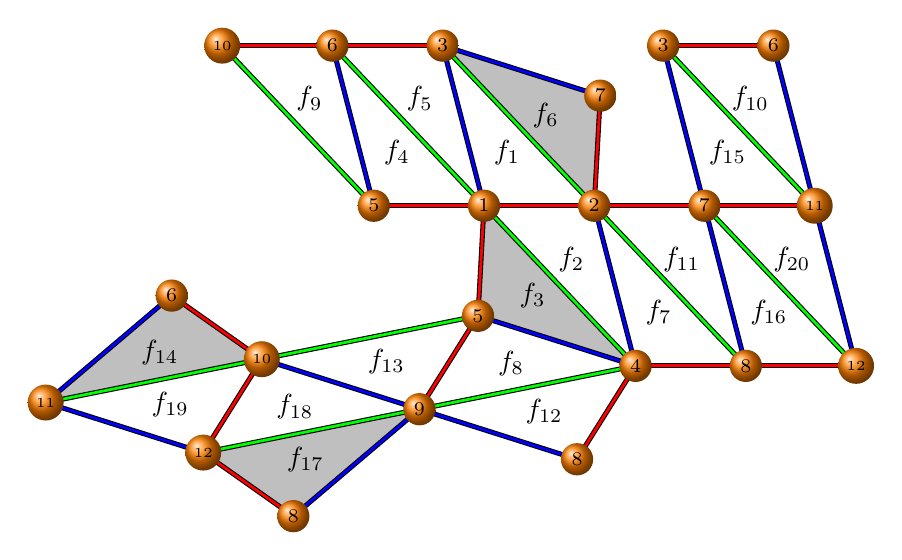
\begin{tikzpicture}[scale=0.7]
            \coordinate (V1_1) at (0, 0);
            \coordinate (V2_1) at (2, 0);
            \coordinate (V3_1) at (-0.75, 2.904737509655563);
            \coordinate (V3_2) at (3.25, 2.904737509655563);
            \coordinate (V4_1) at (2.75, -2.904737509655563);
            \coordinate (V5_1) at (-0.109375, -1.997007037888199);
            \coordinate (V5_2) at (-2, 3.33066907387547e-16);
            \coordinate (V6_1) at (-2.75, 2.904737509655563);
            \coordinate (V6_2) at (5.25, 2.904737509655562);
            \coordinate (V6_3) at (-5.6650390625, -1.630132638882223);
            \coordinate (V7_1) at (2.109375, 1.997007037888199);
            \coordinate (V7_2) at (4, -3.33066907387547e-16);
            \coordinate (V8_1) at (4.75, -2.904737509655563);
            \coordinate (V8_2) at (1.6875, -4.599167723621307);
            \coordinate (V8_3) at (-3.4599609375, -5.631711135256683);
            \coordinate (V9_1) at (-1.171875, -3.691437251853944);
            \coordinate (V10_1) at (-4.75, 2.904737509655564);
            \coordinate (V10_2) at (-4.03125, -2.783706780086581);
            \coordinate (V11_1) at (6, -6.661338147750939e-16);
            \coordinate (V11_2) at (-7.953125000000001, -3.570406522284963);
            \coordinate (V12_1) at (6.75, -2.904737509655564);
            \coordinate (V12_2) at (-5.09375, -4.478136994052326);
            
            
            \fill[white] (V1_1) -- (V2_1) -- (V3_1) -- cycle;
            \node (F1) at (0.4166666666666666, 0.9682458365518543) {$f_{1}$};
            \fill[white] (V1_1) -- (V2_1) -- (V4_1) -- cycle;
            \node (F2) at (1.583333333333333, -0.9682458365518543) {$f_{2}$};
            \fill[lightgray] (V1_1) -- (V4_1) -- (V5_1) -- cycle;
            \node (F3) at (0.8802083333333333, -1.633914849181254) {$f_{3}$};
            \fill[white] (V1_1) -- (V5_2) -- (V6_1) -- cycle;
            \node (F4) at (-1.583333333333333, 0.9682458365518546) {$f_{4}$};
            \fill[white] (V1_1) -- (V3_1) -- (V6_1) -- cycle;
            \node (F5) at (-1.166666666666667, 1.936491673103709) {$f_{5}$};
            \fill[lightgray] (V2_1) -- (V3_1) -- (V7_1) -- cycle;
            \node (F6) at (1.119791666666667, 1.633914849181254) {$f_{6}$};
            \fill[white] (V2_1) -- (V4_1) -- (V8_1) -- cycle;
            \node (F7) at (3.166666666666667, -1.936491673103709) {$f_{7}$};
            \fill[white] (V4_1) -- (V5_1) -- (V9_1) -- cycle;
            \node (F8) at (0.4895833333333333, -2.864393933132569) {$f_{8}$};
            \fill[white] (V5_2) -- (V6_1) -- (V10_1) -- cycle;
            \node (F9) at (-3.166666666666667, 1.936491673103709) {$f_{9}$};
            \fill[white] (V3_2) -- (V6_2) -- (V11_1) -- cycle;
            \node (F10) at (4.833333333333333, 1.936491673103708) {$f_{10}$};
            \fill[white] (V2_1) -- (V7_2) -- (V8_1) -- cycle;
            \node (F11) at (3.583333333333333, -0.9682458365518546) {$f_{11}$};
            \fill[white] (V4_1) -- (V8_2) -- (V9_1) -- cycle;
            \node (F12) at (1.088541666666667, -3.731780828376938) {$f_{12}$};
            \fill[white] (V5_1) -- (V9_1) -- (V10_2) -- cycle;
            \node (F13) at (-1.770833333333333, -2.824050356609574) {$f_{13}$};
            \fill[lightgray] (V6_3) -- (V10_2) -- (V11_2) -- cycle;
            \node (F14) at (-5.883138020833333, -2.661415313751255) {$f_{14}$};
            \fill[white] (V3_2) -- (V7_2) -- (V11_1) -- cycle;
            \node (F15) at (4.416666666666666, 0.9682458365518537) {$f_{15}$};
            \fill[white] (V7_2) -- (V8_1) -- (V12_1) -- cycle;
            \node (F16) at (5.166666666666666, -1.936491673103709) {$f_{16}$};
            \fill[lightgray] (V8_3) -- (V9_1) -- (V12_2) -- cycle;
            \node (F17) at (-3.241861979166667, -4.600428460387651) {$f_{17}$};
            \fill[white] (V9_1) -- (V10_2) -- (V12_2) -- cycle;
            \node (F18) at (-3.432291666666667, -3.65109367533095) {$f_{18}$};
            \fill[white] (V10_2) -- (V11_2) -- (V12_2) -- cycle;
            \node (F19) at (-5.692708333333333, -3.610750098807956) {$f_{19}$};
            \fill[white] (V7_2) -- (V11_1) -- (V12_1) -- cycle;
            \node (F20) at (5.583333333333333, -0.9682458365518549) {$f_{20}$};
            
            
            \tikzset{EdgeStyle/.style = {thin, double distance=1pt} }
            
            \draw[ EdgeStyle, double=red] (V2_1) -- (V1_1);
            \draw[ EdgeStyle, double=blue] (V1_1) -- (V3_1);
            \draw[ EdgeStyle, double=green] (V4_1) -- (V1_1);
            \draw[ EdgeStyle, double=red] (V5_1) -- (V1_1);
            \draw[ EdgeStyle, double=red] (V1_1) -- (V5_2);
            \draw[ EdgeStyle, double=green] (V1_1) -- (V6_1);
            \draw[ EdgeStyle, double=green] (V3_1) -- (V2_1);
            \draw[ EdgeStyle, double=blue] (V2_1) -- (V4_1);
            \draw[ EdgeStyle, double=red] (V7_1) -- (V2_1);
            \draw[ EdgeStyle, double=red] (V2_1) -- (V7_2);
            \draw[ EdgeStyle, double=green] (V2_1) -- (V8_1);
            \draw[ EdgeStyle, double=red] (V6_1) -- (V3_1);
            \draw[ EdgeStyle, double=red] (V3_2) -- (V6_2);
            \draw[ EdgeStyle, double=blue] (V3_1) -- (V7_1);
            \draw[ EdgeStyle, double=blue] (V7_2) -- (V3_2);
            \draw[ EdgeStyle, double=green] (V3_2) -- (V11_1);
            \draw[ EdgeStyle, double=blue] (V4_1) -- (V5_1);
            \draw[ EdgeStyle, double=red] (V8_1) -- (V4_1);
            \draw[ EdgeStyle, double=red] (V4_1) -- (V8_2);
            \draw[ EdgeStyle, double=green] (V4_1) -- (V9_1);
            \draw[ EdgeStyle, double=blue] (V5_2) -- (V6_1);
            \draw[ EdgeStyle, double=red] (V9_1) -- (V5_1);
            \draw[ EdgeStyle, double=green] (V5_2) -- (V10_1);
            \draw[ EdgeStyle, double=green] (V10_2) -- (V5_1);
            \draw[ EdgeStyle, double=red] (V10_1) -- (V6_1);
            \draw[ EdgeStyle, double=red] (V6_3) -- (V10_2);
            \draw[ EdgeStyle, double=blue] (V6_2) -- (V11_1);
            \draw[ EdgeStyle, double=blue] (V11_2) -- (V6_3);
            \draw[ EdgeStyle, double=blue] (V7_2) -- (V8_1);
            \draw[ EdgeStyle, double=red] (V7_2) -- (V11_1);
            \draw[ EdgeStyle, double=green] (V7_2) -- (V12_1);
            \draw[ EdgeStyle, double=blue] (V8_2) -- (V9_1);
            \draw[ EdgeStyle, double=blue] (V9_1) -- (V8_3);
            \draw[ EdgeStyle, double=red] (V12_1) -- (V8_1);
            \draw[ EdgeStyle, double=red] (V8_3) -- (V12_2);
            \draw[ EdgeStyle, double=blue] (V9_1) -- (V10_2);
            \draw[ EdgeStyle, double=green] (V9_1) -- (V12_2);
            \draw[ EdgeStyle, double=green] (V11_2) -- (V10_2);
            \draw[ EdgeStyle, double=red] (V12_2) -- (V10_2);
            \draw[ EdgeStyle, double=blue] (V11_1) -- (V12_1);
            \draw[ EdgeStyle, double=blue] (V12_2) -- (V11_2);
            
            
            
            \tikzset{VertexStyle/.style = {
             shape = circle,
             ball color = orange,
             text = black,
             inner sep = 2pt,
             outer sep = 0pt,
             minimum size = 8pt} }
            
            \node[VertexStyle] at (V1_1) {\scriptsize 1};
            \node[VertexStyle] at (V2_1) {\scriptsize 2};
            \node[VertexStyle] at (V3_1) {\scriptsize 3};
            \node[VertexStyle] at (V3_2) {\scriptsize 3};
            \node[VertexStyle] at (V4_1) {\scriptsize 4};
            \node[VertexStyle] at (V5_1) {\scriptsize 5};
            \node[VertexStyle] at (V5_2) {\scriptsize 5};
            \node[VertexStyle] at (V6_1) {\scriptsize 6};
            \node[VertexStyle] at (V6_2) {\scriptsize 6};
            \node[VertexStyle] at (V6_3) {\scriptsize 6};
            \node[VertexStyle] at (V7_1) {\scriptsize 7};
            \node[VertexStyle] at (V7_2) {\scriptsize 7};
            \node[VertexStyle] at (V8_1) {\scriptsize 8};
            \node[VertexStyle] at (V8_2) {\scriptsize 8};
            \node[VertexStyle] at (V8_3) {\scriptsize 8};
            \node[VertexStyle] at (V9_1) {\scriptsize 9};
            \node[VertexStyle] at (V10_1) {\tiny 10};
            \node[VertexStyle] at (V10_2) {\tiny 10};
            \node[VertexStyle] at (V11_1) {\tiny 11};
            \node[VertexStyle] at (V11_2) {\tiny 11};
            \node[VertexStyle] at (V12_1) {\tiny 12};
            \node[VertexStyle] at (V12_2) {\tiny 12};

        \end{tikzpicture}
        }
\end{frame}

\begin{frame}{Embedded icosahedron}
    \begin{minipage}{0.45\textwidth}
        \includegraphics[width=\textwidth]{DSC09508.JPG}
    \end{minipage}
    \begin{minipage}{0.45\textwidth}
        \includegraphics[width=\textwidth]{DSC09510.JPG}
    \end{minipage}
\end{frame}
            

\begin{frame}{Further research}
    \begin{itemize}
        \pause
        \item Structural properties of coloured surfaces
        \pause
        \item Embedding of surfaces into $\R^3$
        \pause
        \item Folding of surfaces (description and classification)
        \pause
        \item GAP--implementation of this theory
    \end{itemize}

    \pause
    \vfill
    \begin{center}
        {\LARGE Thanks for your attention}
    \end{center}

    \vfill
    {\small
    Alice Niemeyer \hfill Markus Baumeister

    Wilhelm Plesken \hfill Ansgar Strzelczyk
    }
\end{frame}


\end{document}
